\chapter{Experimentación y Resultados}
    Aquí se presentaran los resultados del \textbf{Análisis a Posteriori} de cada algoritmo solicitado.
    
\section{Algoritmo 1}
    El algoritmo codificado en \textit{Python} fue testeado en un entorno virtual de Linux, donde pudimos obtener resultados del mejor caso, peor caso y del algoritmo funcionando en su totalidad normal. 
    \subsection{Mejor Caso}
        Para el mejor caso definimos que la coincidencia se encontrará justo en el primer elemento de cada arreglo. Esto ocasiona que el algoritmo ejecute sus ciclos una sola vez ya que la condición dentro del ciclo \textit{for} terminaría el programa. 
        En la gráfica podemos observar que aunque el tamaño del arreglo cambie el numero de operaciones es constante, lo cual da una linea recta desplazada desde el número de operaciones hasta el arreglo con n=100.
        
        \begin{figure}[htp!]
            \centering
            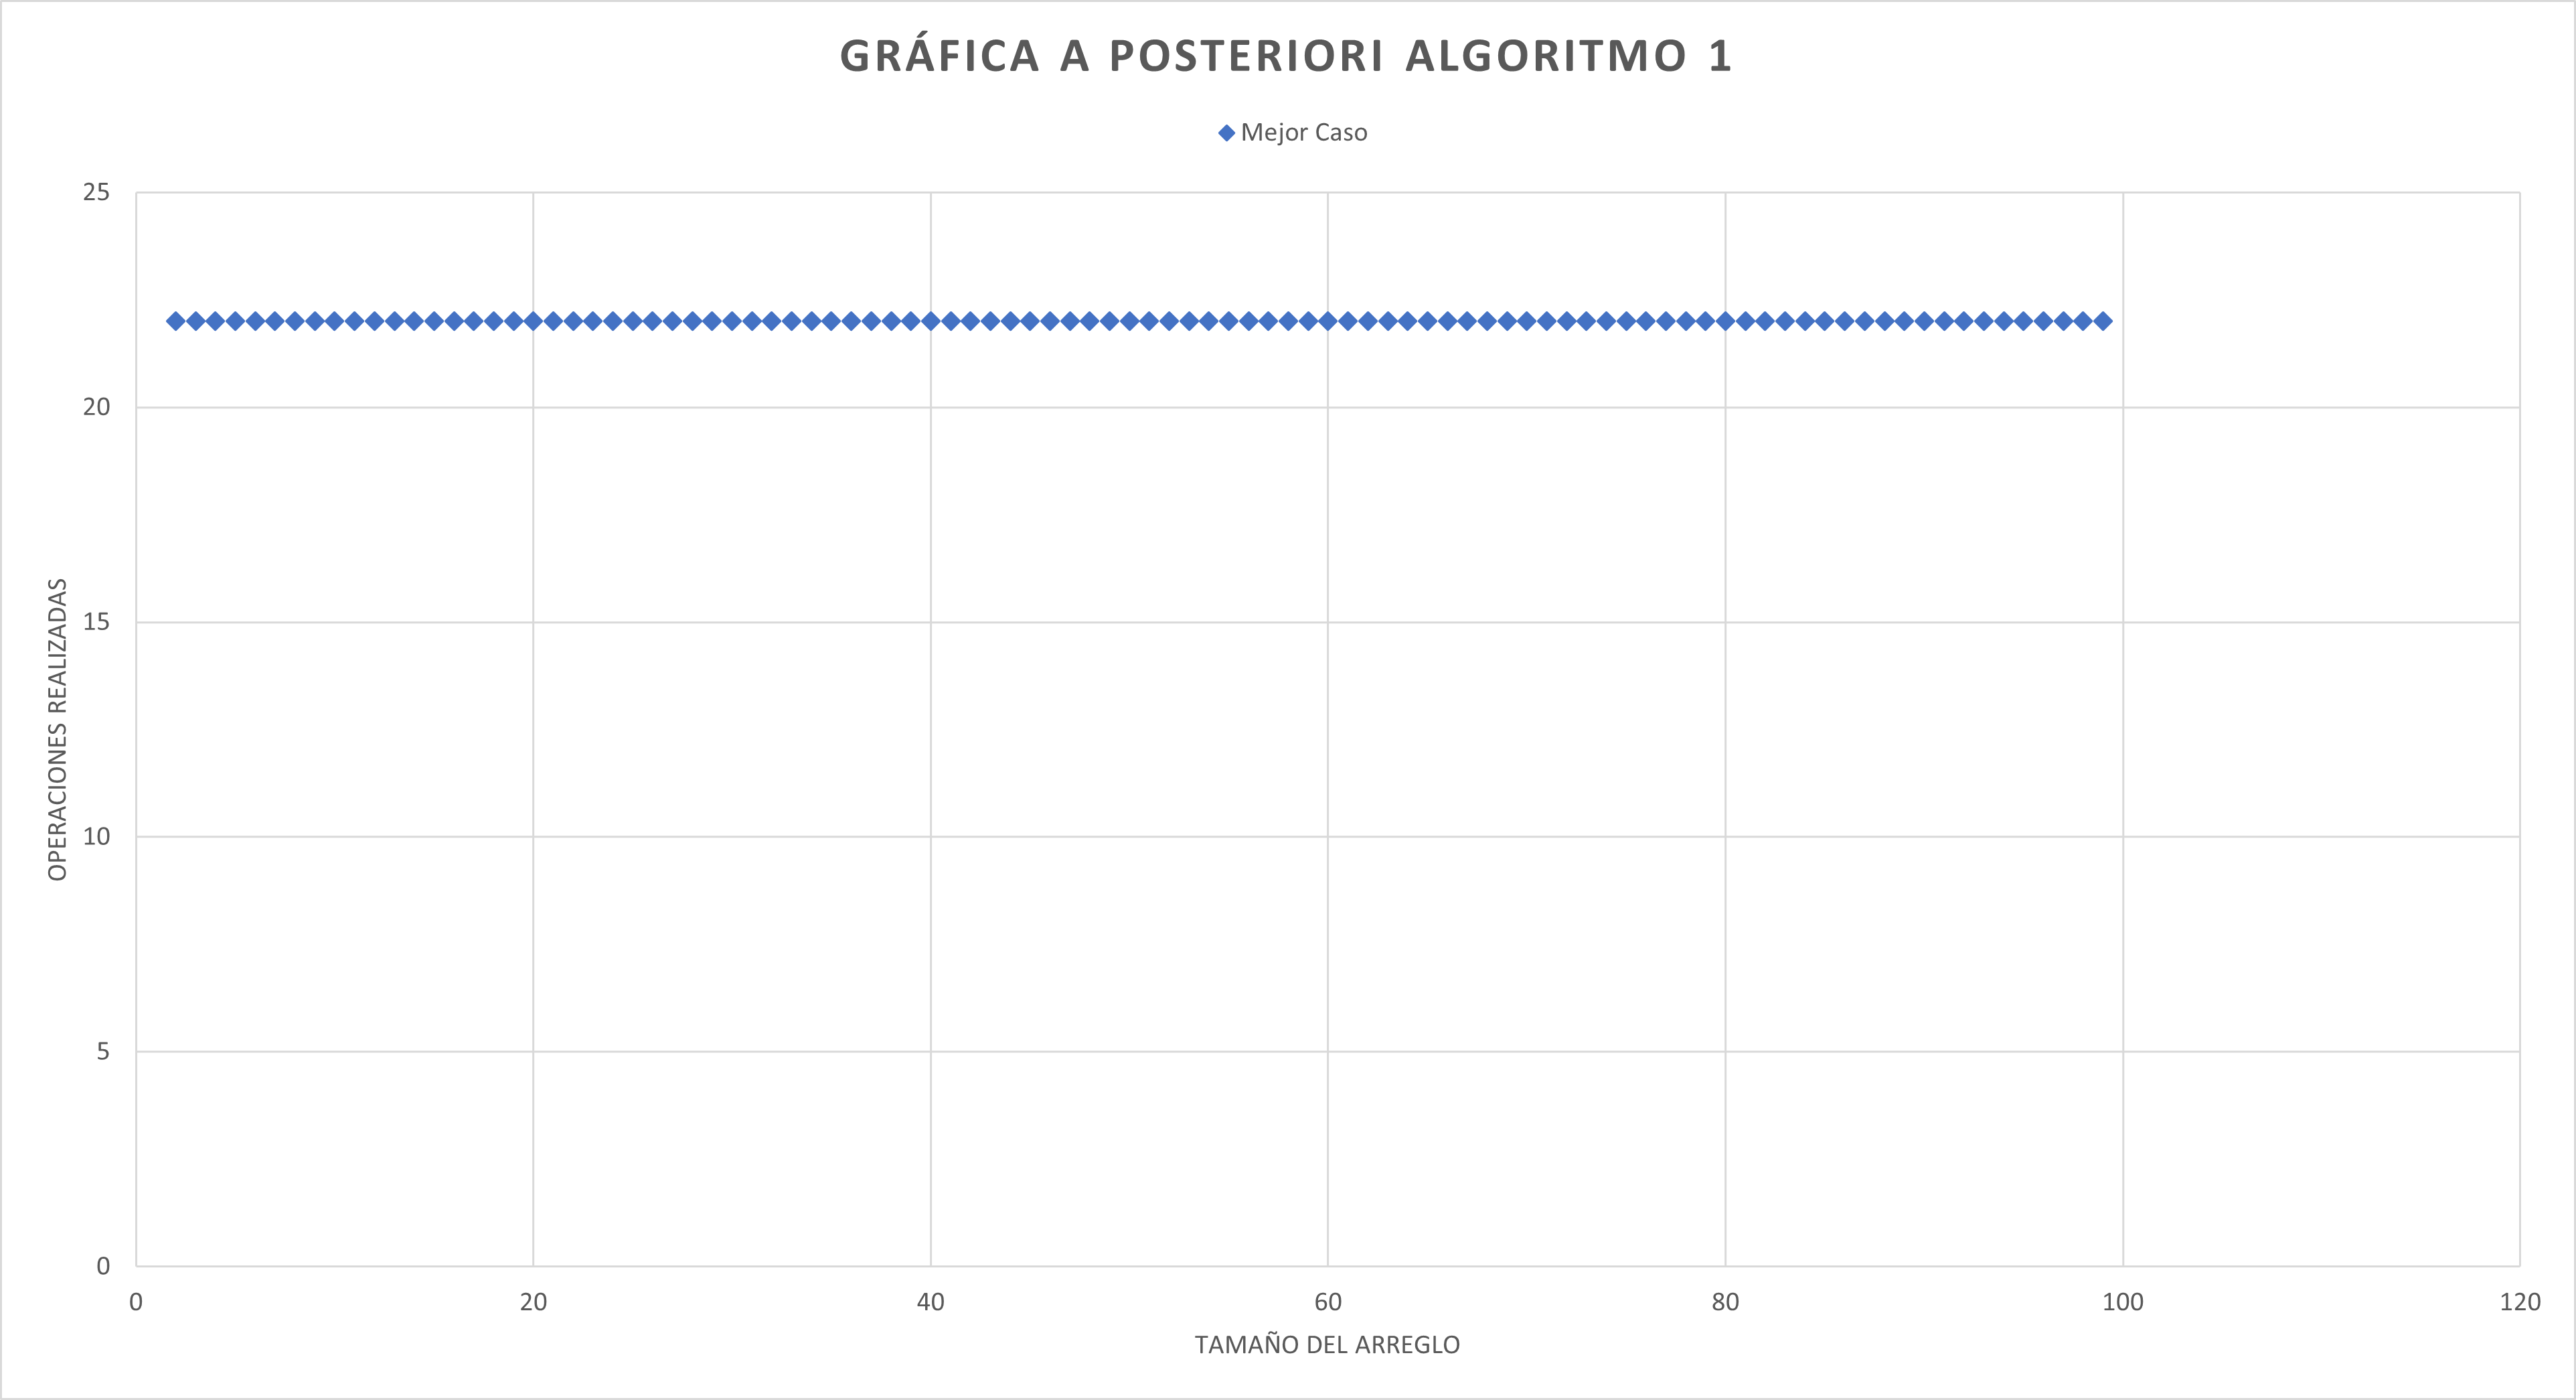
\includegraphics[width=0.8 \textwidth]{Images/Graf_MejorCaso.png}
            \caption{Gráfica Mejor Caso}
            \label{fig:my_label}
        \end{figure}
    
        
    \subsection{Peor Caso}
        En el Peor Caso, definimos que sería cuando no haya ninguna coincidencia en los dos arreglos, lo que ocasionaría que conforme el arreglo incremente su tamaño en n, los pasos ejecutados serán cada vez mayores, ya que al recorrer ambos arreglos y no encontrar nada, se convertiría en un sin fin de pasos. 
        La gráfica muestra esta conclusió con una función cuadratica que parte desde 15 pasos hasta casi 8 mil pasos en el tamaño n=100.
        
        La complejidad del algoritmo es: 
        
        \[\Large{O}(n^2) \]
        
        \begin{figure}[htp!]
            \centering
            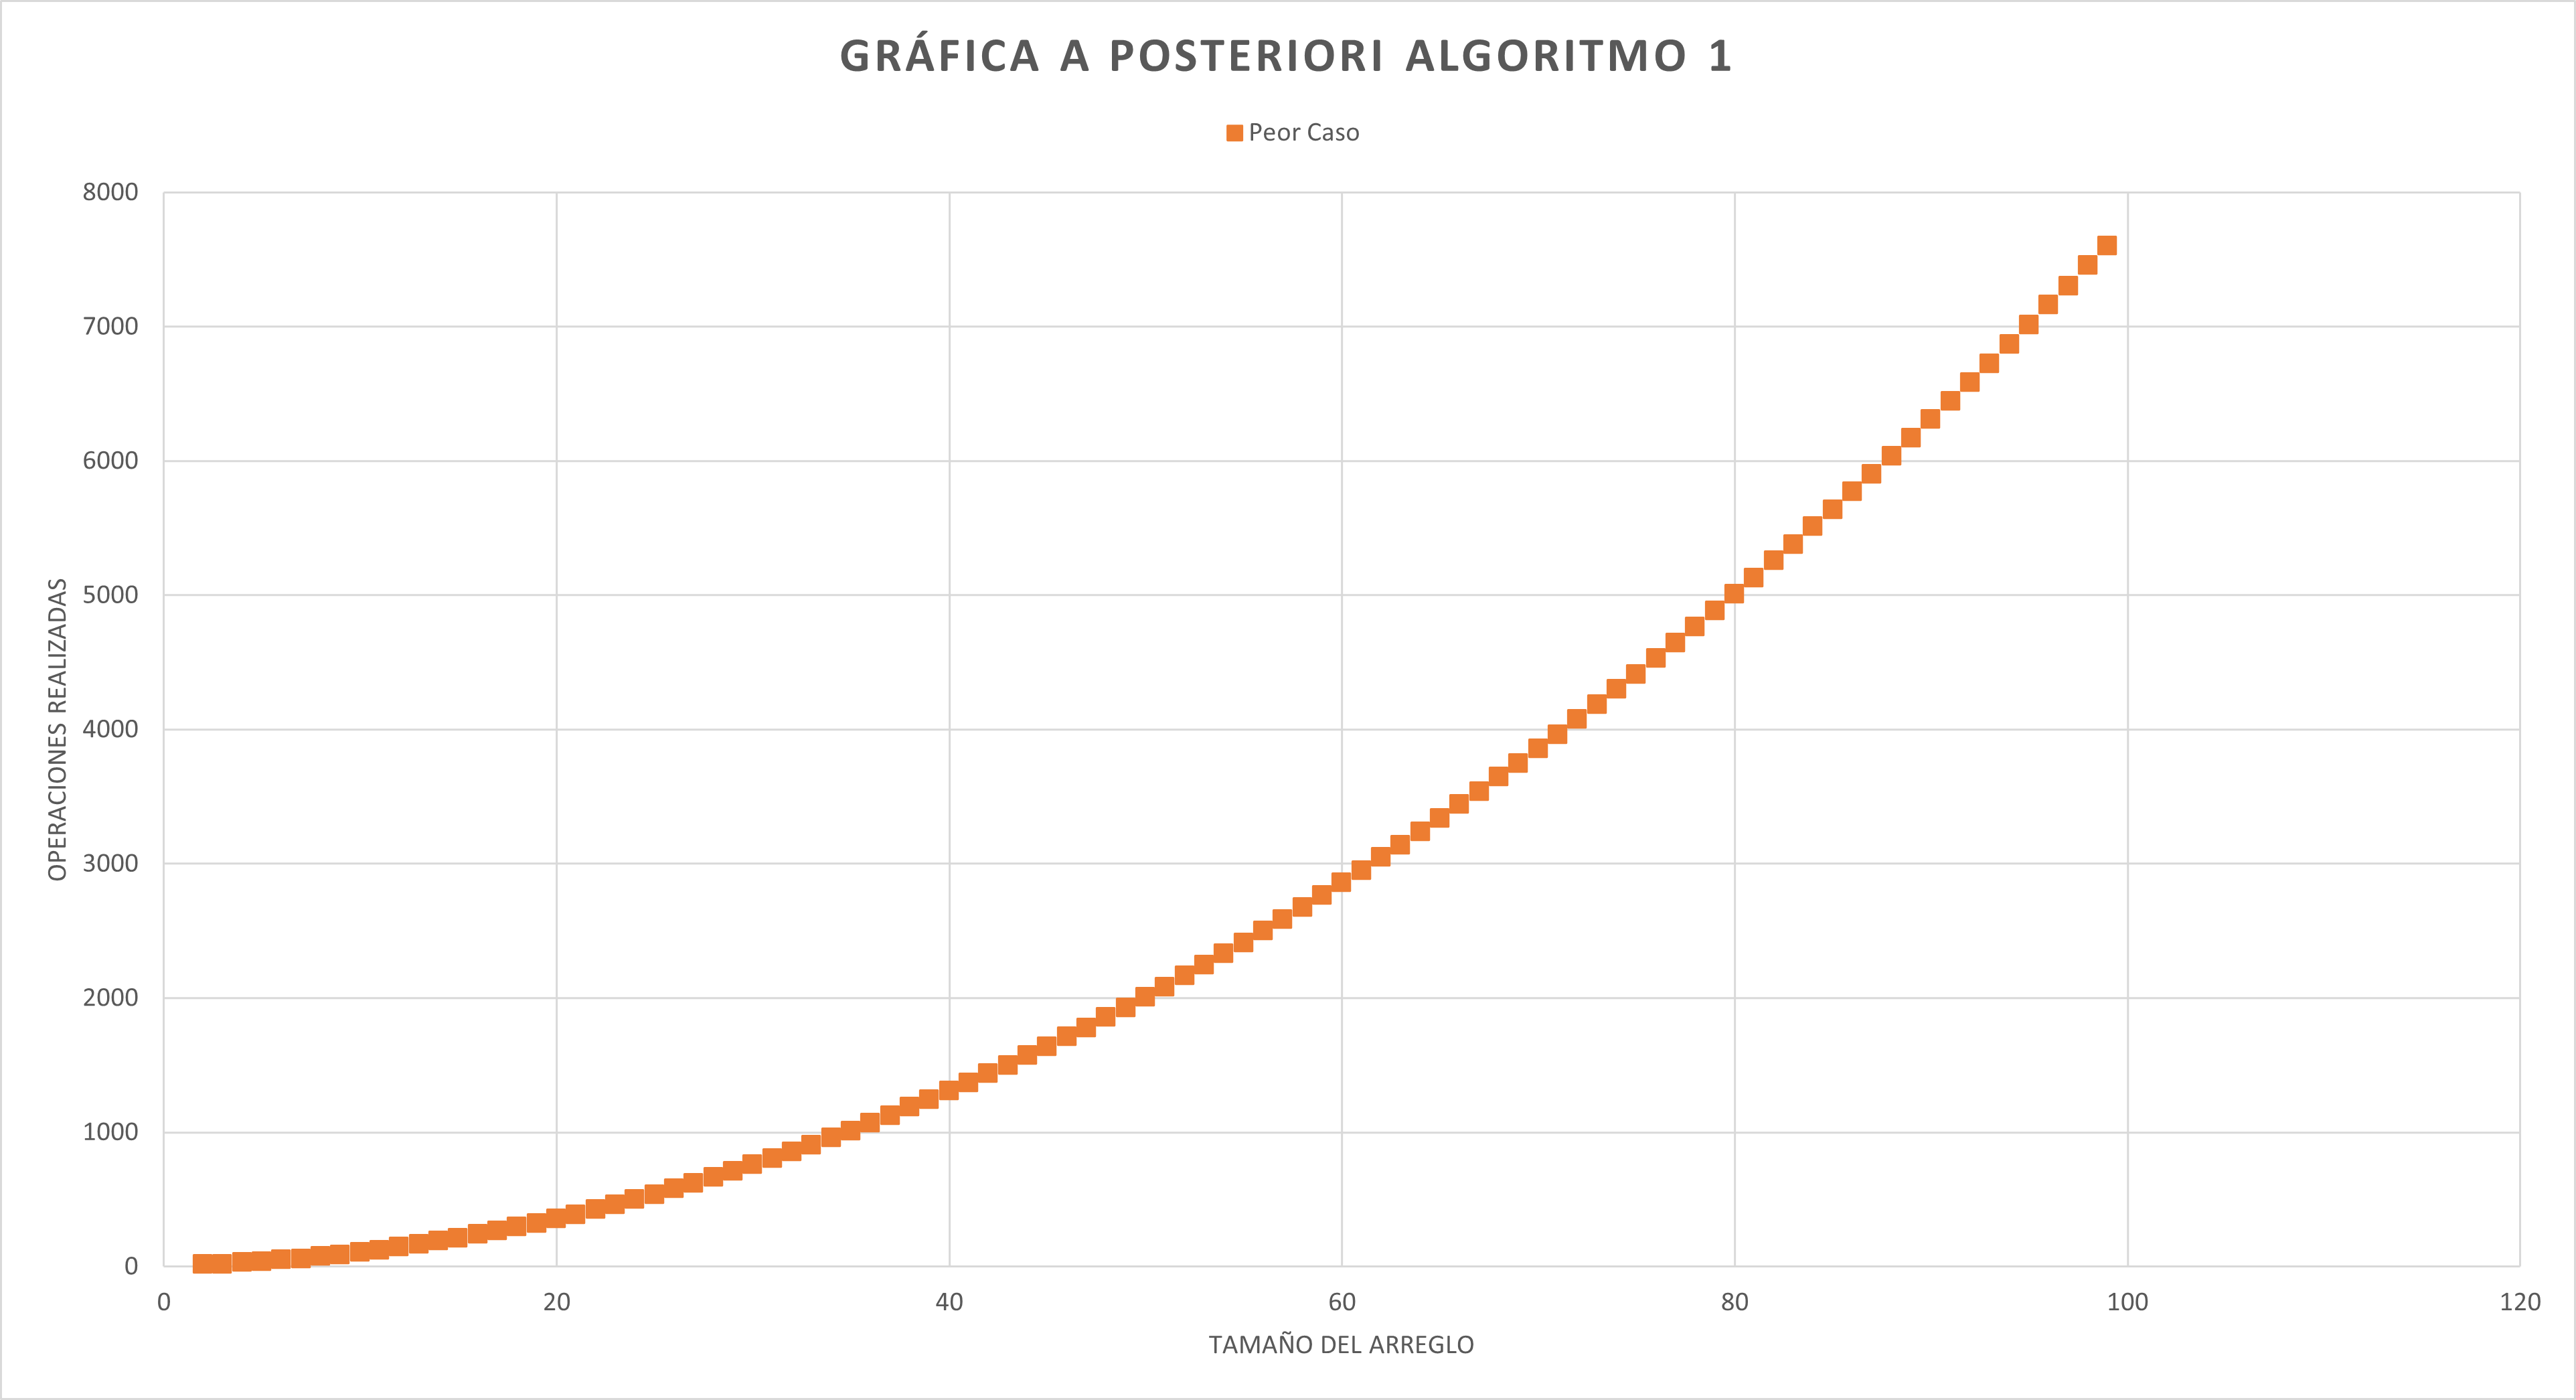
\includegraphics[width=1 \textwidth]{Images/Graf_PeorCaso.png}
            \caption{Gráfica Peor Caso}
            \label{fig:my_label}
        \end{figure}
    
    \newpage
    \subsection{Análisis Normal}
        Obteniendo datos del algoritmo evaluado de manera "normal", podemos atestiguar que entre las cotas el algoritmo funciona de manera adecuada, siendo que tiende a un avance de pocas operaciones mientras escala de tamaño.
        
        \begin{figure}[htp!]
            \centering
            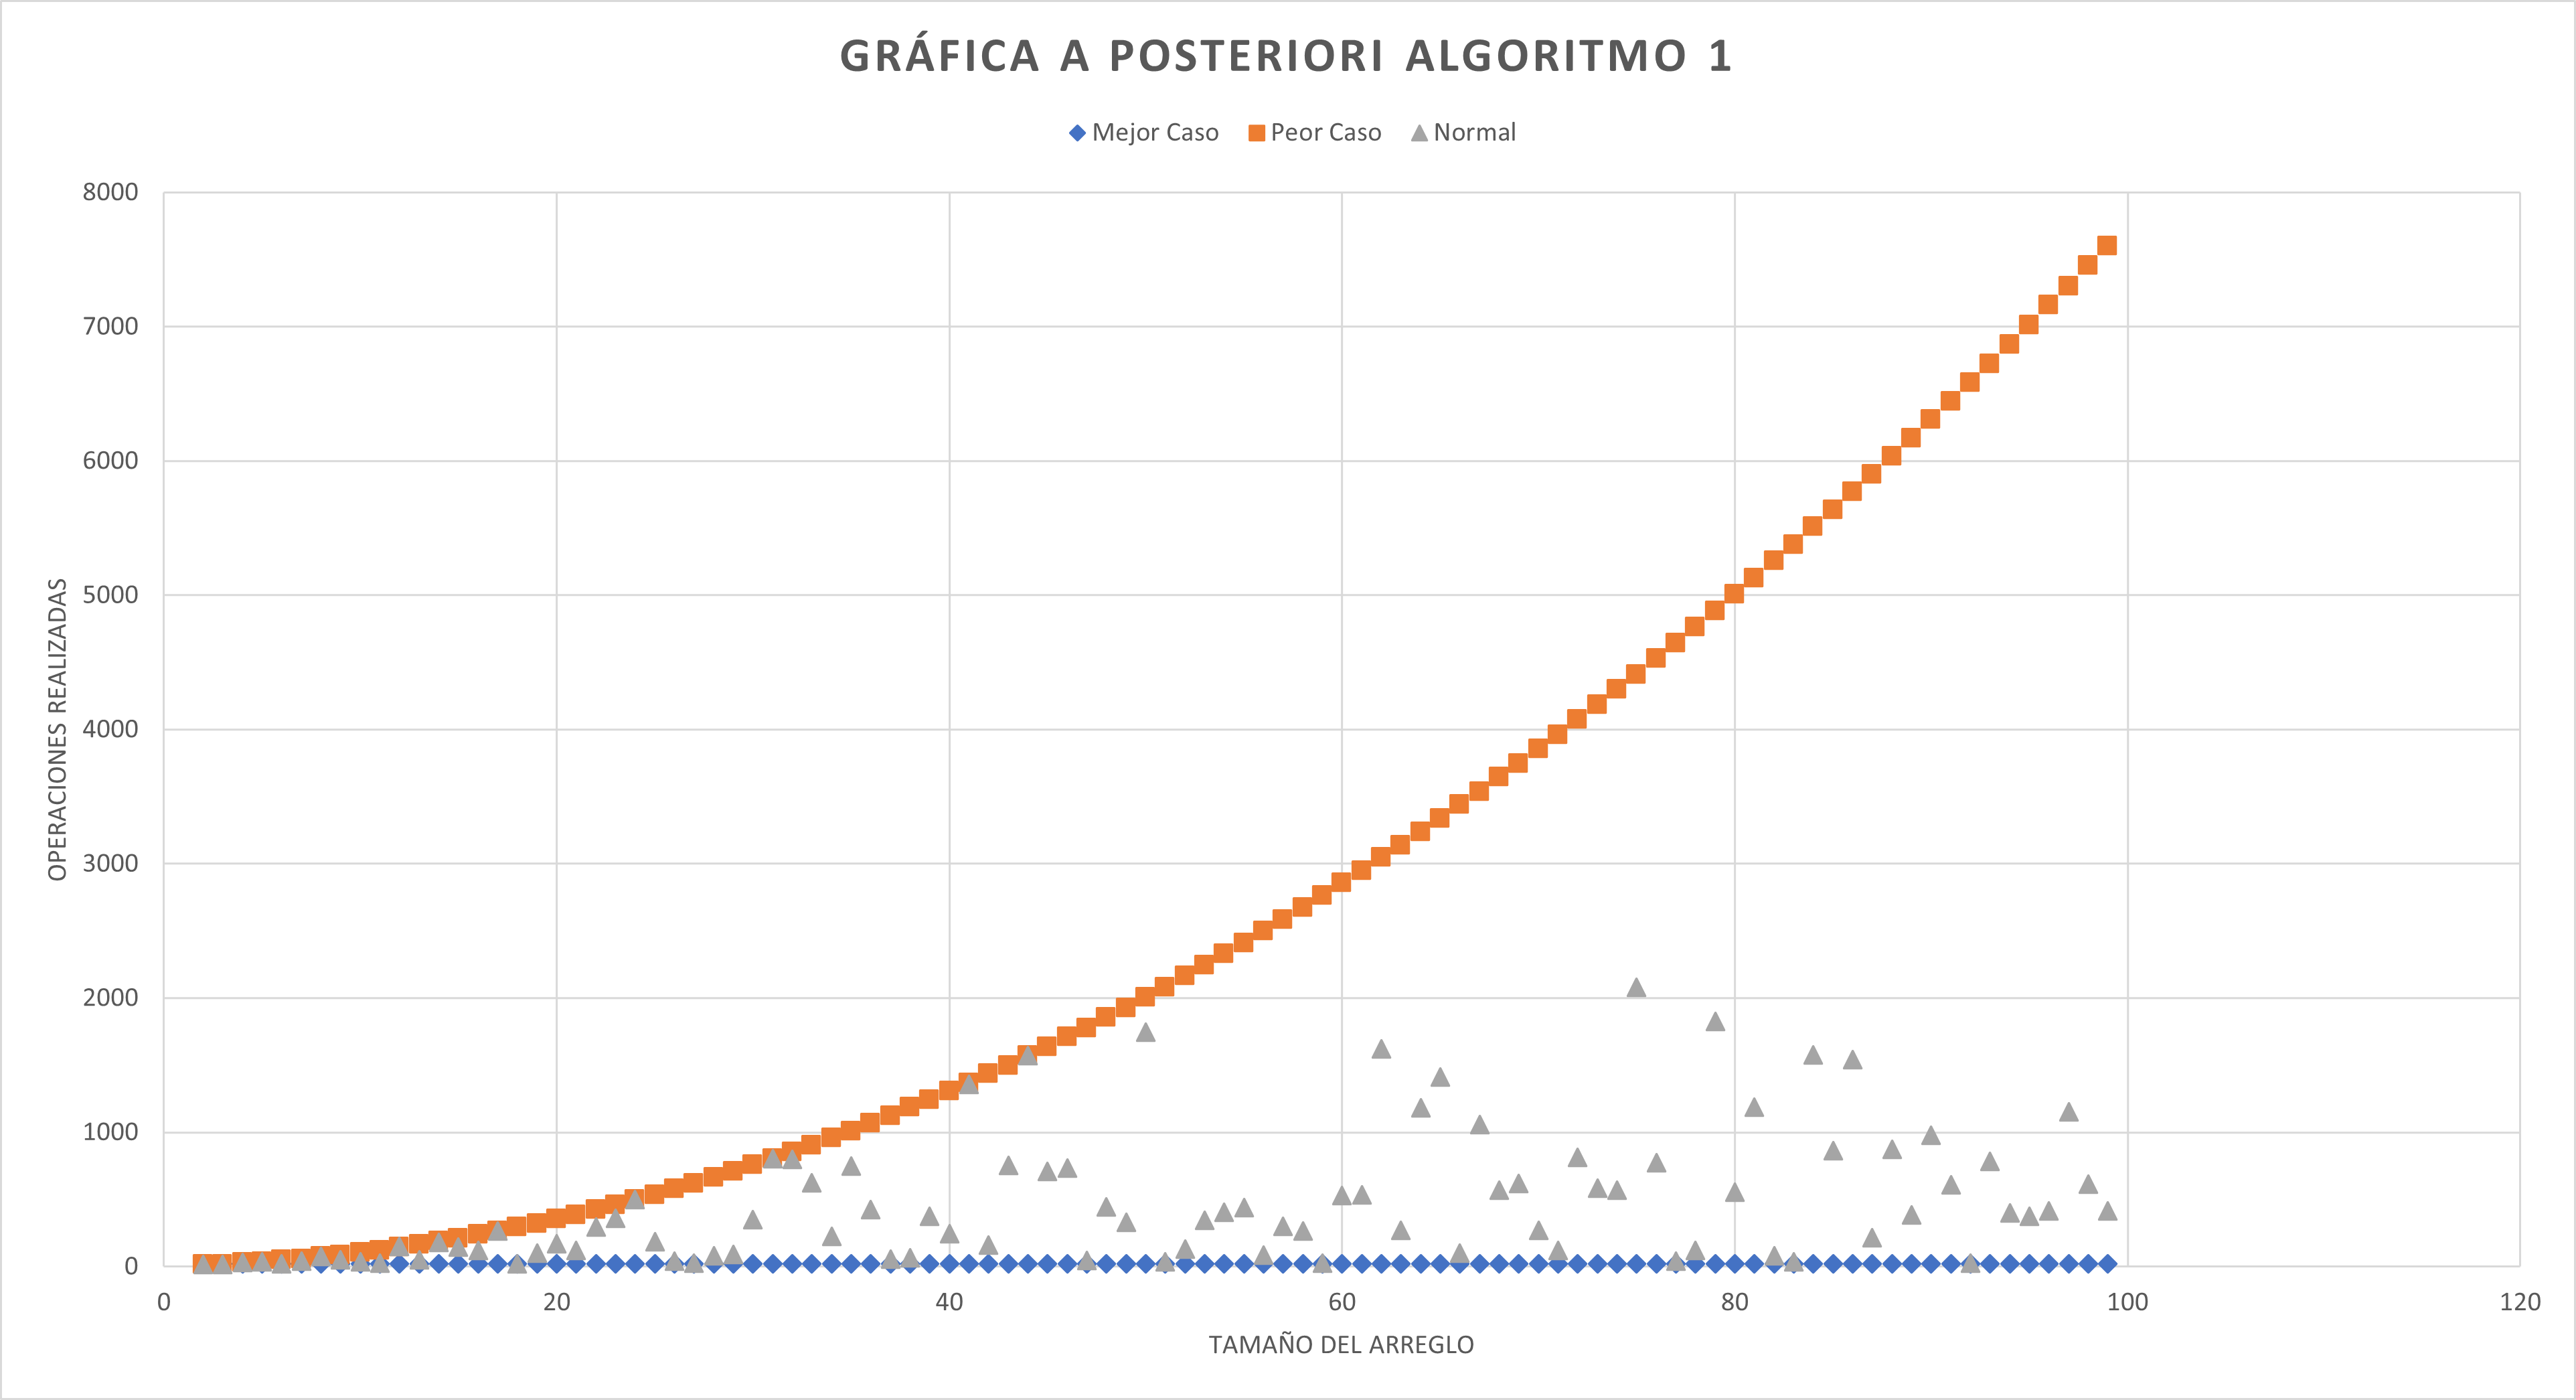
\includegraphics[width=1 \textwidth]{Images/Graf_Normal.png}  
            \caption{Gráfica Algoritmo 1}
            \label{fig:my_label}
        \end{figure}
    
    \newpage
    \section{Algoritmo 2}
        El algoritmo de Euclides fue codificado en \textit{Python}, compilado en un entorno virtual de Linux donde se pudo observar su comportamiento en el peor caso y en el caso normal. Estos resultados fueron capturados en un archivo \textit{.csv} que posteriormente fueron graficados con la herramienta de Office Excel. 
    
    \subsection{Peor Caso}
        El peor caso considera números enteros positivos consecutivos de la serie de Fibonacci. El resultado de esto nos dio una función logarítmica que desplaza desde el origen hasta el infinito. Esto nos muestra que al principio el algoritmo con la serie de Fibonacci identifica una cantidad grande de MCD que va achicando la cantidad conforme avanza la función.
        Su orden de complejidad es:
        
        \[\Large{O}(\log n) \]
        
        \begin{figure}[htp!]
            \centering
            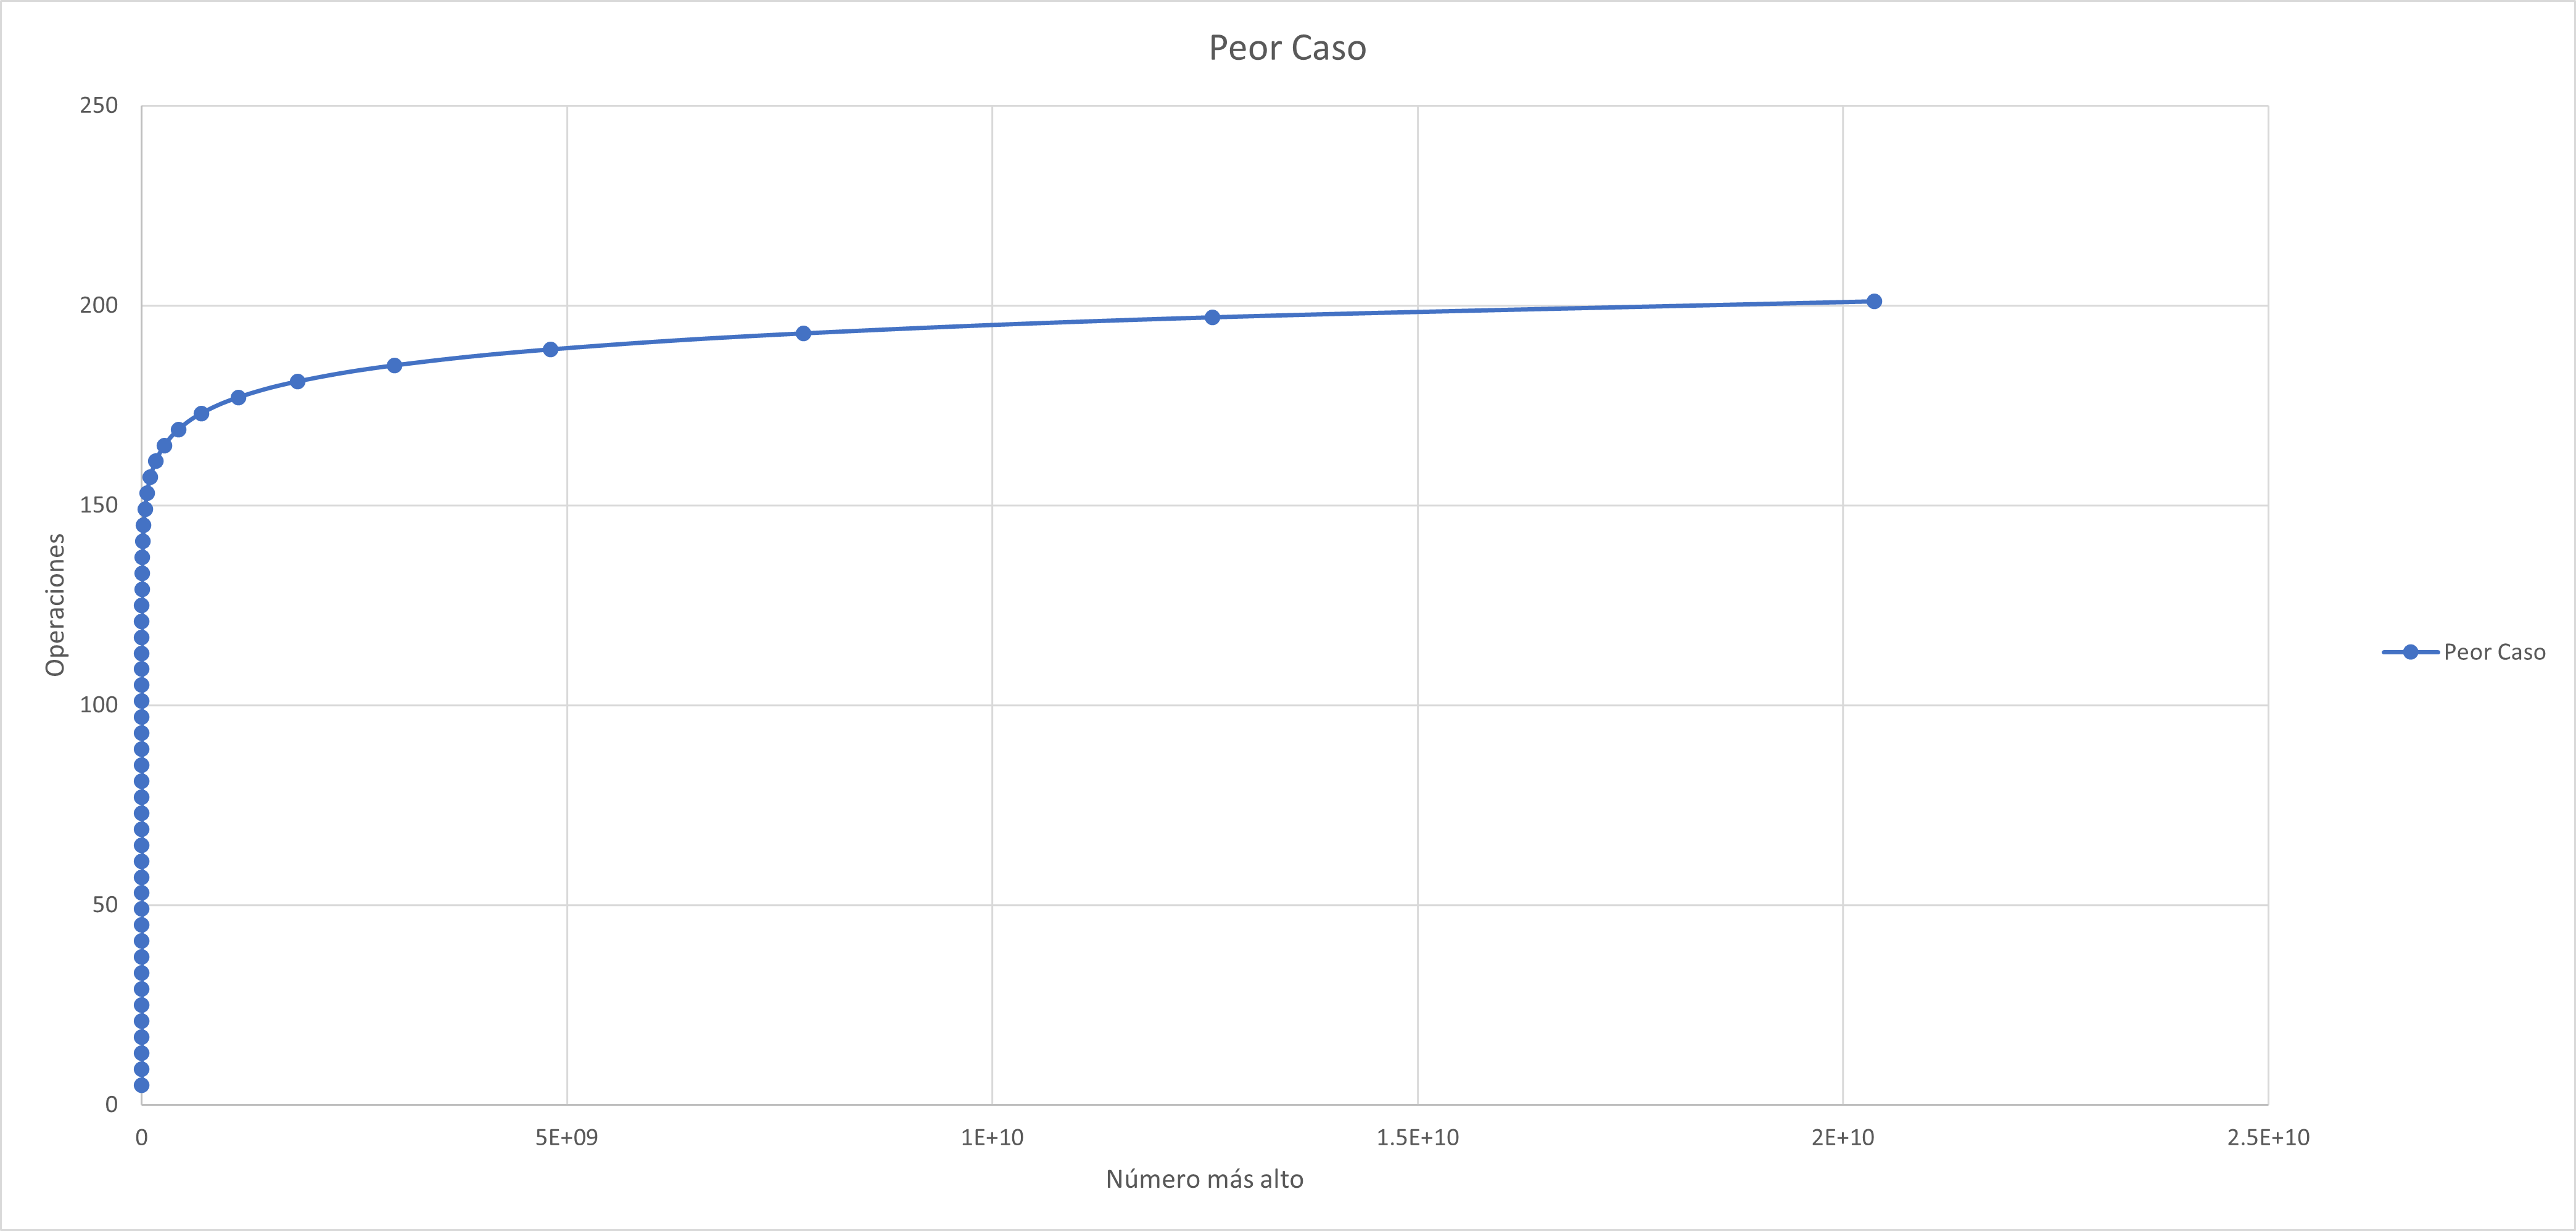
\includegraphics[width=1 \textwidth]{Images/Graf_PeorCaso2.png}  
            \caption{Gráfica Peor Caso}
            \label{fig:my_label}
        \end{figure}
    
    \newpage
    \subsection{Caso Normal}
        Para el caso normal del algoritmo, usamos valores aleatorios entre el 2 y el número máximo del valor del peor caso. El resultado de esto nos dio puntos que se encuentran por debajo de la función logarítmica del peor caso. 
        
        \begin{figure}[htp!]
            \centering
            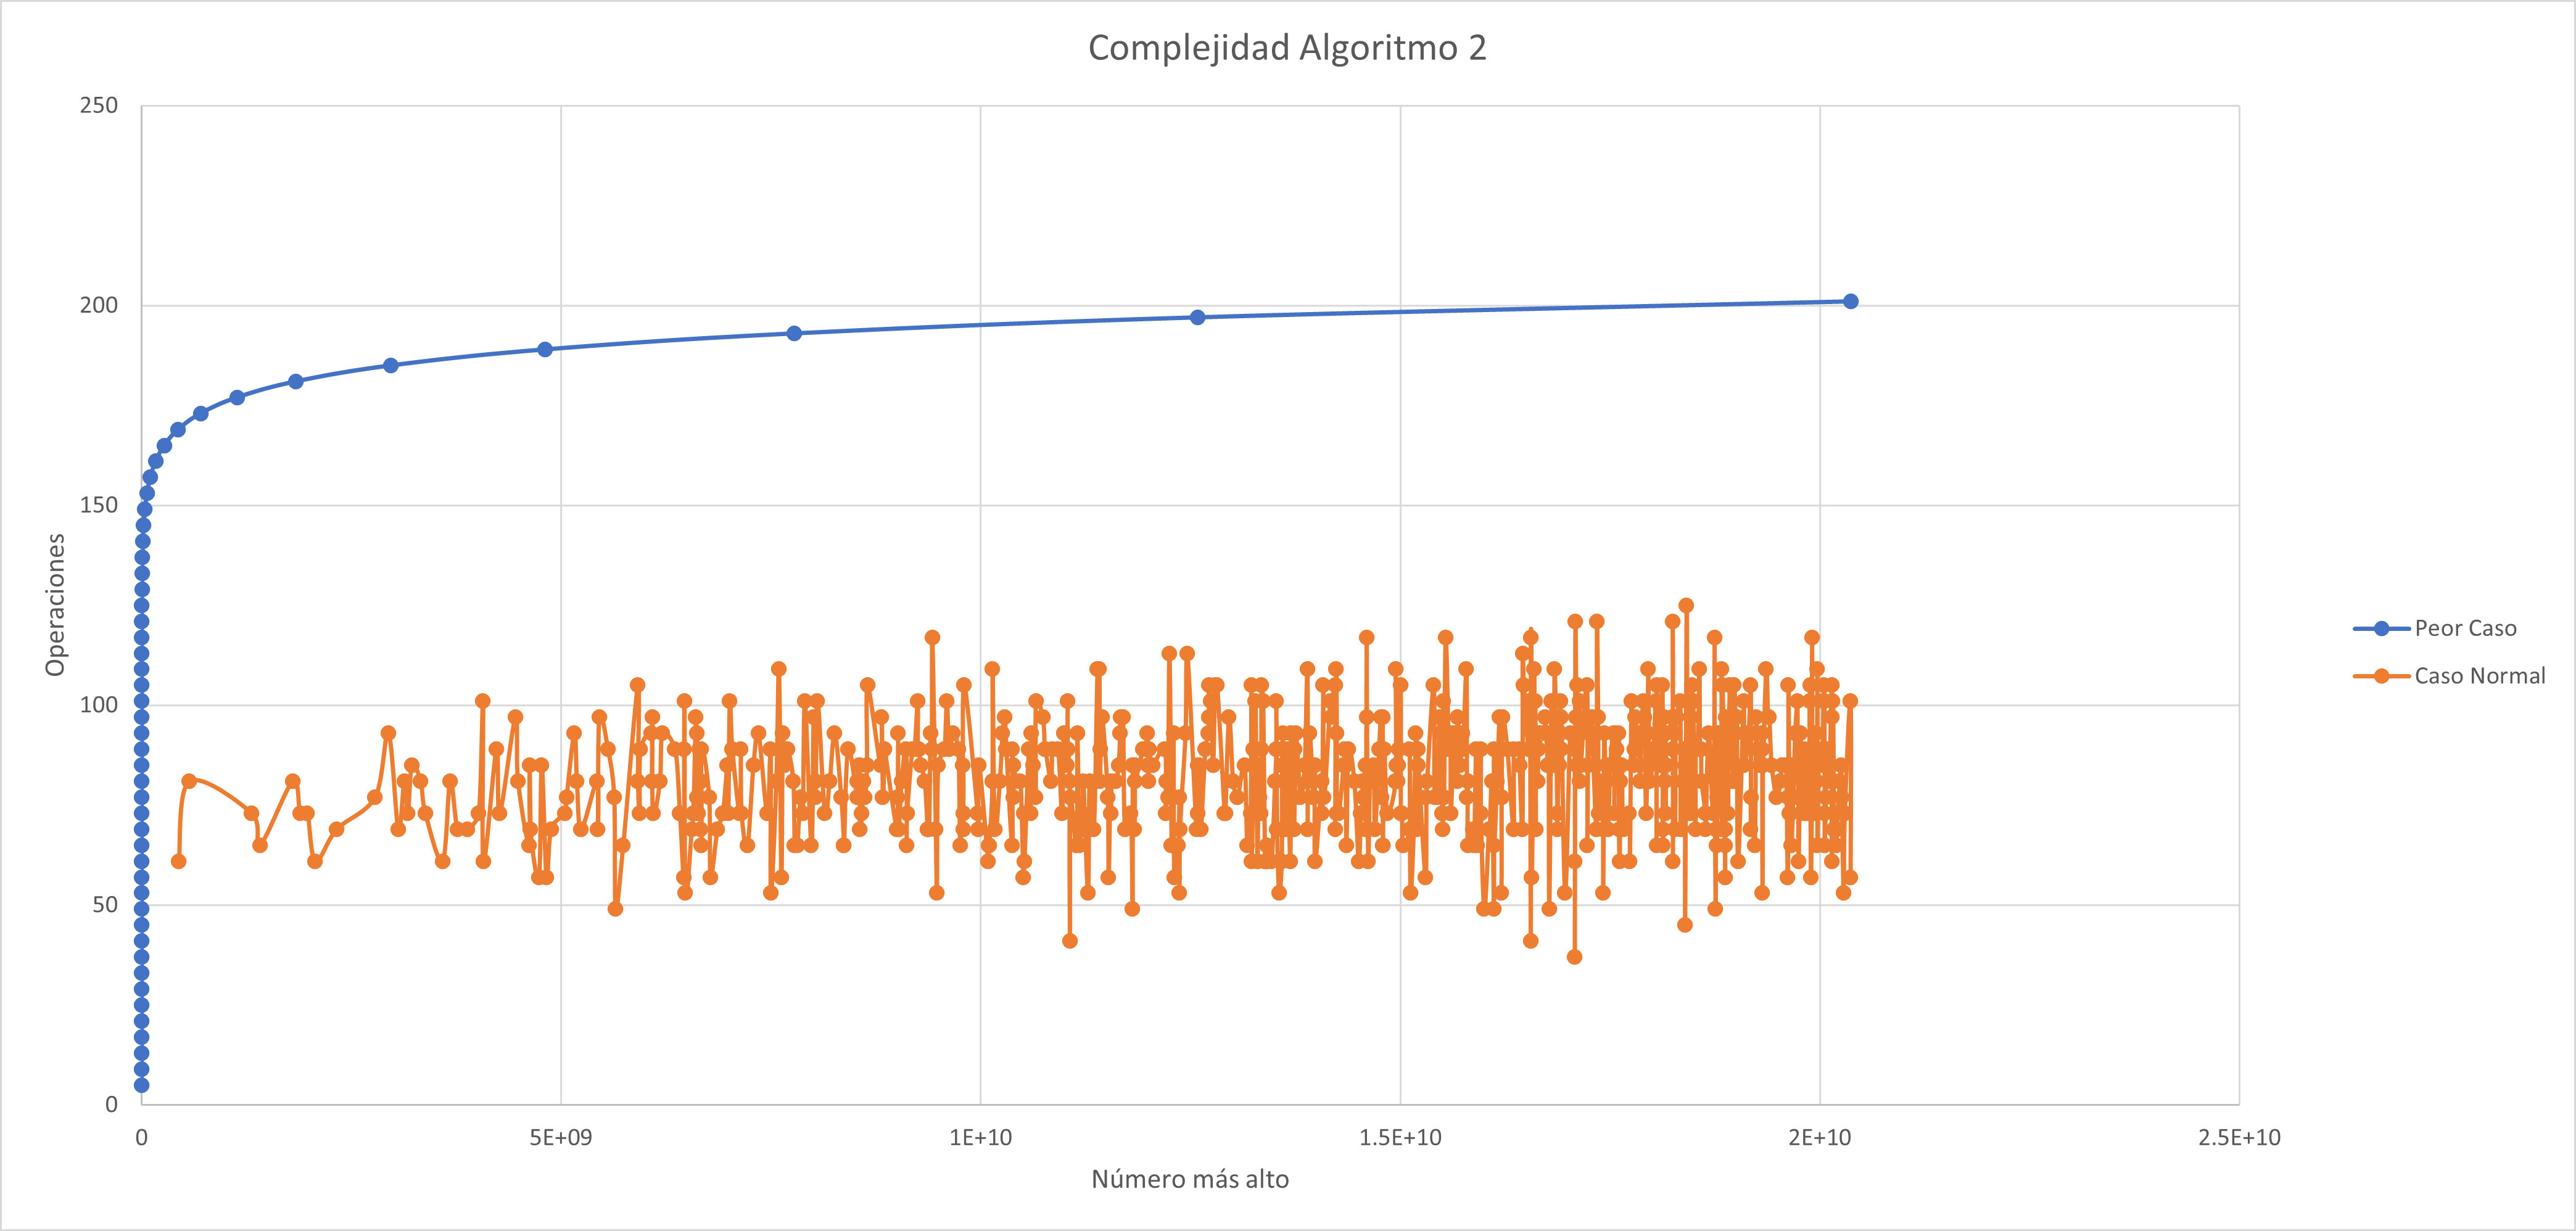
\includegraphics[width=1 \textwidth]{Images/Graf_Normal2.png}  
            \caption{Gráfica Complejidad Algoritmo 2}
            \label{fig:my_label}
        \end{figure}
        
        
    
